\section{Aufbau}
\label{sec:aufbau}


        \begin{figure}
            \centering
            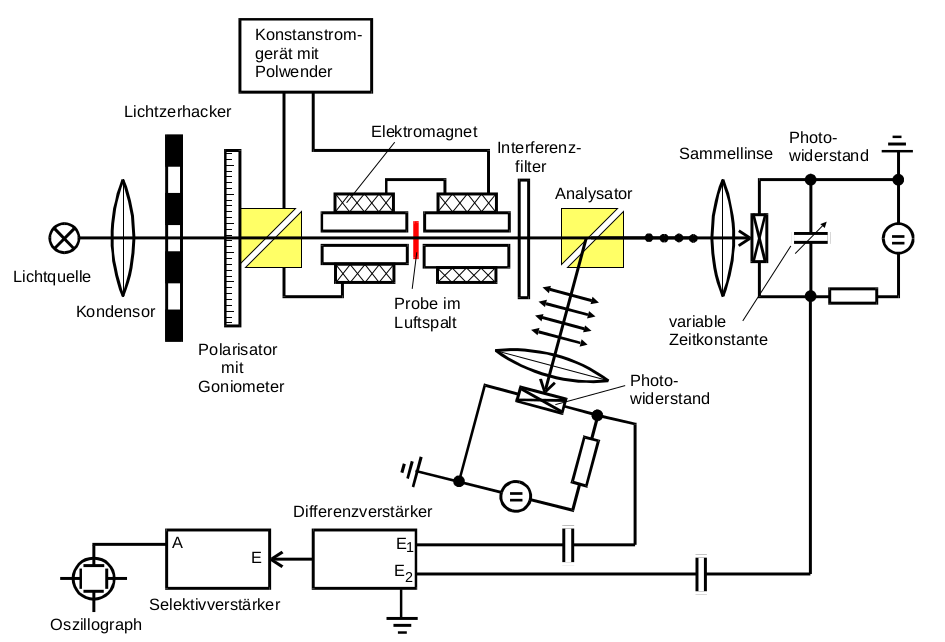
\includegraphics{aufbau.png}
            \caption{Foto des Versuchsaufbaus \cite{tomneu}.}
            \label{fig:aufbau}
        \end{figure}

        Ein Bild des Versuchsaufbaus ist in Abb. \ref{fig:aufbau} zu sehen. 
        Die Quelle der $\gamma-$Strahlung ist eine $\ce{^{137}Cs}-$Quelle.
        Der Strahl wird kollimiert und auf einen 3\,x\,3\,x\,3\,cm\,-Würfel gegeben. 
        Im Experiment werden vier verschiedene Würfel untersucht. 
        Von diesen Würfeln ist einer mit Luft gefüllt und von einer 1\,mm dicken 
        Aluminiumwand umgeben.
        Würfel zwei und drei bestehen nur aus je einem 
        Material, welches durch den Versuch ermittelt wird, und werden 
        ebenfalls von einer Aluminiumwand umrahmt. 
        Der vierte Würfel, welcher die Kennzeichnung "5" trägt, 
        besteht aus 27 1x1-Würfeln, die aus unbekannten Materialien
        zusammengesetzt sind. Für die mittlere Ebene des Würfels, 
        welche aus 9 kleinen Einzelwürfeln besteht, soll die genaue 
        Zusammensetzung ermittelt werden. Auch um diesen Würfel 
        ist eine Aluminiumwand.